\documentclass[10pt,twoside,openright]{memoir}
\usepackage[paperwidth=4.25in, paperheight=6.875in,bindingoffset=.75in]{geometry}
\usepackage[utf8]{inputenc} % If utf8 encoding                                  
\usepackage[T1]{fontenc}    %                                                   
\usepackage[english]{babel} % English please                                    
\usepackage[final]{microtype} % Less badboxes 
\usepackage{tgpagella}
\usepackage{caption}
\usepackage{graphicx}
\usepackage{rotating}

\makeevenhead{headings}%
    {\thepage}{}{}
\makeoddhead{headings}%
    {}{}{\thepage}

\makeatletter
\def\maketitle{%
  \null
  \thispagestyle{empty}%
  \vfill
  \begin{center}\leavevmode
    \normalfont
    {\LARGE\raggedleft \@author\par}%
    \hrulefill\par
    {\huge\raggedright \@title\par}%
    \vskip 1cm
%    {\Large \@date\par}%
  \end{center}%
  \vfill
  \null
  \cleardoublepage
  }
\makeatother

\author{Tao Lin}
\author{Tao Lin}
\title{North American Hamsters}
\date{}










%%% BEGIN DOCUMENT

\begin{document}

\OnehalfSpacing


\let\cleardoublepage\clearpage


\maketitle






\frontmatter


\null\vfill

\begin{flushleft}
\scriptsize
{\em North American Hamsters} is a work of fiction shamelessly stolen from the
internet and reproduced without the author's permission. Names, characters,
places, drugs, MacBooks, grins, and incidents are the product of the author's
imagination or are used fictitiously. Any resemblance to actual persons, 
living or dead (or neither), events, or locales is entirely coincidental. 

\bigskip

Copyright \textcopyright\ 2014 by Tao Lin
\bigskip

Hashtag \#taolin.
\bigskip

All rights reserved. 
\bigskip

Printed in the United States of America by Tony Fader at OfficeMax, a humble
mom-n-pop business located on Capitol Hill in Seattle. 


\end{flushleft}
\let\cleardoublepage\clearpage

\mainmatter
\sloppy

\renewcommand\cftchapteraftersnumb{\normalfont\tiny}
\tableofcontents*




\chapter*{Preface to the 2014 Edition}
\addcontentsline{toc}{chapter}{Preface to the 2014 Edition}
Wow, happy birthday, Allison. Did you know that Tao Lin wrote a series of 
short articles about hamsters, and included hamster illustrations? You're such a
big fan that you probably already knew that. Since you're a big fan, here's a
little booklet of Tao Lin's hamsters. I'd like to think that he wouldn't be 
upset with me for printing this.

\vspace{.5em}
\hspace{7em} {\em Tony Fader} 

\hspace{7em} {\em Seattle, WA}

\chapter*{``Non-Eccentric Piano Prodigy'' Hamster}
\addcontentsline{toc}{chapter}{``Non-Eccentric Piano Prodigy'' Hamster}

Despite being considerably ``less rare'' than the {\em ``Eccentric Piano
Prodigy'' Hamster} (due to a much higher reproduction rate and a more balanced
male-to-female ratio, with there however still being more males than females),
not much is known about the {\em ``Non-Eccentric Piano Prodigy'' Hamster} due to
a near-extreme lack of media coverage and an overall, near-complete lack of
public interest (in terms of the hamster itself; its ``wonderful, crisp, and
tender''---according to {\em L Magazine}---recordings actually enjoy very
strong sales in a consistent, recession-proof manner). 
\begin{figure}[t!]
\begin{center}

\includegraphics[width=0.9\textwidth]{img/noneccentricpianoprodigy}
\end{center}
\caption*{{\em ``Non-Eccentric Piano Prodigy'' Hamster}.}
\end{figure}
In a 2013 feature article
in {\em The New York Times Magazine} a {\em ``Non-Eccentric Piano Prodigy'' 
Hamster} named John Thomason atypically received extensive coverage---to the 
extent of 5839 words, of which 4794 were, however, focused on the question of 
``exactly
why'' the article's author has ``long harbored the strong
suspicion'' that the specific {\em ``Non-Eccentric Piano Prodigy'' Hamster}
named John Thomason is ``being non-eccentric on-purpose?'' and therefore,
from a certain ``second level'' perspective, actually way more eccentric
than the {\em ``Eccentric Piano Prodigy'' Hamster}, whose eccentricity is
conveyed ``directly, genetically, honestly, and without
irony---without,'' according to the article's author, Janice Mikaela,
``the questionably legitimate post/meta-artfulness that John Thomason has
subtly deployed in his life and work ever since, as far as my research shows, he
was born.'' The feature article included two full-page photographs
and---interspersed throughout---eight smaller photographs (these smaller
ones focused on her eyes, hands, forearms, mouth, forehead, and hair) of Janice
Mikaela, who was previously known primarily for her eccentric behavior at panel
discussions and ``elegantly outrageous'' ({\em Vogue}) hairstyle, instead of
portraits of the pianist, who also was not interviewed or contacted for the
article.

\vspace{2em}

\noindent
\textbf{Hunting Tips:} Approach the {\em ``Non-Eccentric Piano Prodigy''
Hamster} after a concert asking for its autograph---stunning it, as no one 
cares enough to want its autograph. Ask another question---any question---to 
further destabilize the {\em ``Non-Eccentric Piano Prodigy'' Hamster}'s 
perception of reality (that no one is interested in it) in order to cause 
cardiac arrest, effectively ending its life. Finally, at your leisure, place 
it in a plastic baggie. \\

\newpage

\noindent
\textbf{Cooking Tips:} Baste in a paste of olive oil, wakame, hijiki, tamari 
at a low heat, ``moving it around'' occasionally. Serve over a thick---but not
 too thick---bed of lettuce. Great with red wine, diluted carrot juice,
 or---surprisingly---almond milk.


\begin{sidewaystable}
\begin{center}
  \small
  \begin{tabular}{rl}
  \textbf{Average weight/height (record)} & .9 lbs/3.3" (1.6 lbs/3.9") \\
  \textbf{Average life expectancy (record)} & 18.4 years (36.9 years) \\
  \textbf{Favorite book(s)} & {\em The Mind of God} \\
  \textbf{Favorite band(s)} & anything by Chopin, Brahms \\
  \textbf{Favorite movie(s)} & {\em Eternal Sunshine}  \\
  \textbf{Favorite sexual position} & missionary \\
  \end{tabular}
\end{center}
\caption*{{\em``Non-Eccentric Piano Prodigy'' Hamster} facts.}
\end{sidewaystable}

\chapter*{Factory-Farmed Hamster}
\addcontentsline{toc}{chapter}{Factory-Farmed Hamster}
Force-fed intravenously for the last four days of its eighteen-day,
regimentally/existentially genocidal lives of ``allegory-like'' ``extreme,
sustained, increasing pain,'' the {\em Factory-Farmed Hamster} is by-far the
most common hamster in North America, with a population expected to exceed 200
billion by 2020, a number expected, henceforth, to grow at a rate of 26.4\% per
year, as fast-food companies expand to third-world countries. Born in darkness
in a space not large enough for it to turn around without doing a kind of
back-flip, the {\em Factory-Farmed Hamster} lives its next three days/nights in
a mostly-unconscious haze of bone-level inflammation and intermittent paralysis,
sometimes reflexively jerking forward/backward .5 to .8 inches to prevent its
lower body from ``crystallizing'' in an advanced form of atrophy, while being
force-fed every four hours a mixture of non-organic corn, metastasized
fecal-matter, industrial-strength antibiotics, 4 to 9 varieties of growth
hormones. The next eleven days the {\em Factory-Farmed Hamster} is force-fed
pellets containing the meat/bones/tumors/fur of ``fellow, deceased'' {\em
Factory-Farmed Hamsters} grinded---along with their ``waste,'' which often is
scientifically ``not discernable'' from their ``bodies''---into paste-like
matter that is ``marinated'' 4-8 hours in an antibiotic-hormone mixture and then
dehydrated in gigantic microwaves. 
\begin{figure}[t!]
\begin{center}
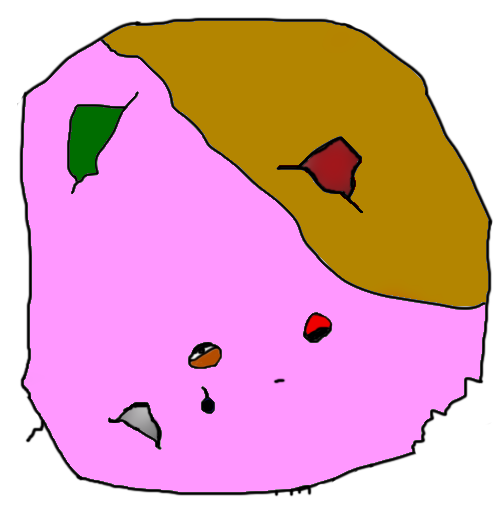
\includegraphics[width=0.9\textwidth]{img/factoryfarmed}
\end{center}
\caption*{{\em Factory-Farmed Hamster}.}
\end{figure}
For the final four days of its ``surreally
bleak existence'' ({\em Mother Jones}) the {\em Factory-Farmed Hamster} is moved
into a larger pen and positioned, within rubber canopies, in a manner allowing
its mouth, facing ``upwards,'' to be uncomplicatedly filled, five times a
day, in a kind of ``funneling action,'' in which former migrant farmhands
without passports, in a job with a 37\% long-term survival rate (many ``succumb''
to various cancers after four years), ``funnel'' (a misnomer, as actually a
``tube'' is used) a non-dehydrated form of ``meat/corn paste'' directly into the
stomach of the {\em Factory-Farmed Hamster}, 73\% of which are, scientifically,
``in comas'' by the morning of the fourth day. In 2010 the FDA declared it
governmentally acceptable for meat labeled ``grade-A'' to continue to be
force-fed up to 35 hours after its source is ``no longer conscious,'' increasing
profits by 18\%. In America an emerging, popular conspiracy theory is that
factory-farmed meat is harmful to those who eat it; connected to or ``in support
of'' that conspiracy, some say, is the taboo, or ``feeling of
shame/inauthenticity/[something],'' of buying organic food, which itself is
related, some say, to the vaguely embarrassing, or ``offensive,'' even, choice
to spend more money on [anything] than ``the lowest amount possible''---a
feeling caused, perhaps, to some degree, by vague intuitions of ```taking part'
in `the conspiracy,' '' along with the influence of the powerful abstraction
most people ultimately convey in the form of the word ``bourgeoisie,'' according
to one conspiracy theorist whose YouTube videos were deleted by YouTube after
pressure from the FDA, who acted ``in preemption,'' according to a fourth-party
conspiracy theorist (whose YouTube videos were also deleted but have since
reappeared on Vimeo), to pressure from the meat/dairy industry.

\noindent
\textbf{Hunting Tips:} Wearing a military-grade gas mask and a
full-body-coverage suit made of space-grade polymers (to protect against deadly
skin lesions and tumors, which have been known to ``fly off'' {\em
Factory-Farmed Hamsters}, when hit by metal doors or simply when they
``burst''), cut a small hole in the corner of a factory-farm shed at night.
Place the {\em Factory-Farmed Hamster} in a garbage bag or shoebox, as it will
not fit in a plastic baggie, taking care not to collapse from empathy-induced
``intense depression'' or ``fear of `evil' in the world,'' as the {\em
Factory-Farmed Hamster} will likely appear ``horrifyingly grotesque'' (Stephen
King via {\em Esquire}), be blind, likely ``crying.''

\vspace{1em}
\noindent
\textbf{Cooking Tips:} Sprinkling antibiotics continuously, grind in entirety
after soaking in a bowl of hydrogen peroxide for 5 to 8 hours. Boil with garlic,
dehydrate, condense into pellets for fish food or ``little balls'' for dog or
cat food. Add [anything] for bulk, grind with antibiotics, and resell to
international or outsourced factory farms as ``grade-A factory farm feed,'' to
second/third-world countries as ``meal packets,'' or fourth-party dog food
producers as ``all-natural, high-grade dog food guaranteed to give your
pet's fur a healthy sheen.''

\begin{sidewaystable}
\begin{center}
  \small
  \begin{tabular}{rl}
  \textbf{Average weight/height (record)} & 4.4 lbs/4.2" (4.8 lbs/4.6") \\
  \textbf{Average life expectancy (record)} & .049 years (.049 years) \\
  \textbf{Favorite book(s)} & doesn't know what a ``book'' is \\
  \textbf{Favorite band(s)} & doesn't know what a ``band'' is \\
  \textbf{Favorite movie(s)} & doesn't know what a ``movie'' is \\
  \textbf{Favorite sexual position} & doesn't know what ``sex'' is \\
  \end{tabular}
\end{center}
\caption*{{\em Factory-Farmed Hamster} facts.}
\end{sidewaystable}

\chapter*{``Unable to Process Neutral Statements as Neutral'' Hamster}
\addcontentsline{toc}{chapter}{``Unable to Process Neutral Statements as Neutral'' Hamster}
Widespread, ``to the point of rampancy,'' some say---not inaccurately, as it can
``indeed'' be found on every continent---but concentrated most densely in the
United States and other etiologically British populations, the {\em``Unable to
Process Neutral Statements as Neutral'' Hamster}, or {\em Unableham}, views
nearly all hamster-caused phenomenon (and most natural phenomenon, also, to some
degree) as strongly and defaultedly rhetorical. In a 2012 study of over ten
thousand {\em Unablehams} 94\% identified the sentence ``I went to Wal-Mart,
bought a black shirt and two bananas, paid with my HSBC debit card'' as directly
conveying one of the following: ``America's consumerist economy is destructive
and amoral'' (54\%), ``generation [whatever the current generation is labeled]
suffers from a non-European form of `ultimately inauthentic' ennui unique to
its historical/cultural/technological context'' (20\%), ``Banana Republic's
labor tactics are shameful and fascist'' (11\%), ``the government should
bail-out banks but only in times of severe, potentially long-term, international
crisis'' (9\%). An ``astounding, simply astounding'' ({\em Village Voice}) 63\%
said they would refer to the sentence in a court of law, under oath, if asked,
as ``scathing.'' 
\begin{figure}[t!]
\begin{center}

\includegraphics[width=0.9\textwidth]{img/unableham}
\end{center}
\caption*{{\em ``Unable to Process Neutral Statements as Neutral'' Hamster}.}
\end{figure}
A follow-up study designed to test the extent of the {\em
Unableham}'s genetic inability to interpret reality without framing it in a
personal, hierarchal, often ``strongly opinionated'' system found that 39\%
interpreted the Atlantic Ocean as ``against the Bourgeoisie'' and 47\%
interpreted the Mona Lisa as ``one of the strongest elements of propaganda
against the unfair treatment of women workers in late 19th century America since
Chopin's second Ballade, the one in F Major'' (due to a lack of funding the
study was also designed to test the ability of hamsters to discern ``since''
statements in sentences where the chronology is grammatically illogical).
Cross-breeds well with {\em Shit-Talking Hamsters} and, surprisingly, {\em
Freshwater Hamsters}.

\noindent
\textbf{Hunting Tips:} Approach it in a manner somehow ``indisputably friendly,''
employing a level of sarcasm that causes ``strong discomfort,'' if needed, as
you force the muscles on your face into certain configurations---effectively
overpowering, if successful, the Unableham's ``subconscious, possibly
uncontrollable'' cognitive mode of ``continuously replacing the metaphysical
perspective of others with one's own metaphysical perspective,'' causing it to
view your demeanor as ``amiable,'' to some degree, so that maybe it will move
toward you slightly. Repeat until the desired specimen is ``in range.'' Place it
in a plastic baggie.

\vspace{1em}
\noindent
\textbf{Cooking Tips:} Shave, rinse, cut into 5-10 chunks---optionally, 
deep-freeze, at this point, for a more chicken-like consistency---and dip in an
egg-and-butter-based mixture, coating each chunk evenly/completely, before
sprinkling cornstarch on them. Carefully immerse in a vat of hot oil, the oil of
your choice. Serve with steamed broccoli or waffle fries.

\begin{sidewaystable}
\begin{center}
  \small
  \begin{tabular}{rl}
  \textbf{Average weight/height (record)} & 1.4 lbs/3.6'' (1.8 lbs/4.1'') \\
  \textbf{Average life expectancy (record)} & 12.2 years (31.4 years) \\
  \textbf{Favorite book(s)} & {\em Life of Pi} \\
  \textbf{Favorite band(s)} & {\em Radiohead} \\
  \textbf{Favorite movie(s)} &  {\em Dances with Wolves} \\
  \textbf{Favorite sexual position} & doggy-style \\
  \end{tabular}
\end{center}
\caption*{{\em ``Unable to Process Neutral Statements as Neutral'' Hamster} 
facts.}
\end{sidewaystable}

\chapter*{Prize-Winning Hamster}
\addcontentsline{toc}{chapter}{Prize-Winning Hamster}

Previously identifiable by the conspicuous growths on the sides of their bodies
that resemble (and, tests have shown, literally are) prize ribbons, many
Prize-Winning Hamsters have, in the past three years, begun amputating their
ribbons in painless procedures utilizing laser technology first developed for
use in global warfare. (It should also be noted that it's not uncommon, even
for those who can afford the expensive laser procedure, for Prize-Winning
Hamsters to perform DIY surgeries that are often excruciatingly painful and
sometimes fatal.) Today an estimated 38\% of Prize-Winning Hamsters have
de-prized themselves, opting viscerally out of the hierarchy they've been
born into mysteriously. The other 62\% can be identified by prize ribbons ranging
mostly from 1st place to 10th, though rankings as low as the mid 40s (and, once,
649th, which is the lowest on record) have been photographed, usually while the
subject is running away in shame. It's been speculated that Prize-Winning
Hamsters of each ranking---from 1 to 1000---exist in relatively equal
quantity, but that those lower in rank, embarrassed and afraid to be seen, live
deep underground, therefore seem rare or nonexistent. 

\begin{figure}[t!]
\begin{center}

\includegraphics[width=0.9\textwidth]{img/prizewinning}
\end{center}
\caption*{Prize-Winning Hamster.}
\end{figure}

\noindent
\textbf{Hunting Tips:} Prize-Winning Hamsters can be insanely confident (sprinting
through public spaces shouting in joy while flailing its entire body, in extreme
cases) or severely lacking in self-esteem (crying in small, lightless holes
while eating baked goods in scenes of nonhumorous bleakness), depending on the
ranking of their prize ribbon. Approach a specimen ranked high enough (9th or
better is recommended) that it won't immediately escape in fear, placing it
in a plastic baggie.

\vspace{1em}
\noindent
\textbf{Cooking Tips:} Carefully remove the prize ribbon, which can be used in any
situation requiring a prize ribbon of the given ranking. Peel and slice the body
like a kiwi, using the skin and its connective fatty tissue to lightly broil the
body, which can be sliced or made into a paste. For de-prized hamsters, before
doing anything else, excise and discard the scar tissue, which can appear
depressing, or at least distracting, and therefore unappetizing, on an otherwise
consistently contoured piece of meat.

\chapter*{Inconspicuously Hyperlinked Hamster}
\addcontentsline{toc}{chapter}{Inconspicuously Hyperlinked Hamster}

Nondescript unless touched with a force between 18 and 26 psi, causing the
appearance of a dotted line sort of hovering beneath it and a light blue glow
emanating from its surface, indicating it's a hyperlink, or `link',
the Inconspicuously Hyperlinked Hamster is otherwise a fine, vegetarian,
outgoing species of North American hamster---hard-working, considerate,
perceptive, a boon to its ecosystem, with no known allergies or viral
susceptibilities.

\noindent
\textbf{Hunting Tips:} Carefully enclose your own body in not-loose clothing before
getting out of your car, because touching an Inconspicuously Hyperlinked Hamster
at a force exceeding 26 psi (atmospheric pressure is around 14.7 psi at sea
level) will instantly relocate your consciousness out of the vessel of your body
to [unknown], some say. Others, however, say there's no reason to believe
the dotted lines and light blue glows are hyperlinks---that they serve some
other purpose, such as camouflage. Then there are those who focus on how it
seems impossible to prove the presence or non-presence of a consciousness in a
body, therefore it's not possible to detect whether a body's
consciousness has, or has not, been teleported to [unknown]. 

\begin{figure}[t!]                                                              
\begin{center}                                                                  

\includegraphics[width=0.9\textwidth]{img/hyperlinked}                         
\end{center}                                                                    
\caption*{Inconspicuously Hyperlinked Hamster.}                                               
\end{figure}

\noindent
\textbf{Cooking Tips:} Considered a delicacy because of the process of 
delinking that
must be completed before it can be seasoned and eventually ingested,
Inconspicuously Hyperlinked Hamsters appear on the menus of most mid-to-high-end
restaurants around the world. The most common method of delinking is via an
assembly-line process that ends in the hamster being placed in a
higher-dimensional form of MSWord and a worker pushing `Undo Hyperlink'
on a touch-screen.

\end{document}
